\documentclass[12pt,a4paper]{article}
\usepackage{amsmath,amssymb}
\usepackage{booktabs}
\usepackage{geometry}
\usepackage{graphicx}
\usepackage{float}
\usepackage{listings}
\usepackage{xcolor}
\usepackage{algorithm}
\usepackage{algpseudocode}
\usepackage{titlesec}
\usepackage{setspace}
\usepackage{ragged2e}

%----------------------------------------
% Page Setup for A4
%----------------------------------------
\geometry{
  a4paper,
  top=1in,
  bottom=1in,
  left=1in,
  right=1in
}

\setstretch{1.2}

%----------------------------------------
% Section title formatting
%----------------------------------------
\titleformat{\section}
  {\normalfont\bfseries\fontsize{14}{14}\selectfont}
  {\thesection}{1em}{}

%----------------------------------------
% Code listing style
%----------------------------------------
\lstdefinestyle{matlabstyle}{
  language=Matlab,
  basicstyle=\ttfamily\footnotesize,
  keywordstyle=\color{blue}\bfseries,
  commentstyle=\color{green!60!black},
  stringstyle=\color{orange!80!black},
  frame=none,
  numbers=none,
  breaklines=true,
  showstringspaces=false,
  tabsize=2
}

%----------------------------------------
\begin{document}

%----------------------------------------
% Cover Page
%----------------------------------------
\begin{titlepage}
\centering

\vspace*{0.5cm}
\includegraphics[width=0.22\textwidth]{diu_logo.png}\par
\vspace{0.5cm}

{\Large \textbf{Department of Computer Science and Engineering} \par}
\vspace{0.2cm}
{\Large \textbf{Dhaka International University} \par}

\vspace{0.8cm}

{\normalsize
Semester: 12th \par
Lab Report No: 04 \par
Course Code: CSE-420 \par
Course Title: Image Processing Lab \par
Report Title: Fourier Transform, Frequency Domain Filtering, and Bit Plane Slicing in MATLAB \par
}

\vspace{1cm}

{\Large \textbf{Submitted By} \par}
\vspace{0.3cm}

{\normalsize
Rasheduzzaman Rakib \par
Reg. No.: CS-D-77-22-120080 \par
Roll: 37 \par
Batch: D-77 \par
Department of Computer Science and Engineering \par
Dhaka International University \par
}

\vspace{1cm}

{\Large \textbf{Submitted To} \par}
\vspace{0.3cm}

{\normalsize
Md. Muksit Ul Islam \par
Assistant Professor \par
Department of Computer Science and Engineering \par
Dhaka International University \par
}

\vfill

{\normalsize Submission Date: 25th September 2026 \par}
{\normalsize Summer 2026 \par}

\end{titlepage}


%----------------------------------------
% Lab Report
%----------------------------------------

\section{Name}

\textbf{Fourier Transform, Frequency Domain Filtering, and Bit Plane Slicing in MATLAB}\\[0.3em]
Topics covered: Fourier Transform (FFT), Magnitude Spectrum, Ideal Low Pass Filter,
Ideal High Pass Filter, Bit Plane Slicing.

%----------------------------------------

\section{Description}

This lab covers frequency domain analysis and bit-level decomposition of digital
images in MATLAB. The cameraman.tif image is used for FFT and filtering operations,
while peppers.png is used for bit plane slicing.

\begin{enumerate}
  \item \textbf{Fourier Transform (FFT):} The 2D Fast Fourier Transform converts
        a spatial-domain image into its frequency-domain representation using
        fft2. The result is centred using fftshift so that the DC component
        appears at the middle of the spectrum.

  \item \textbf{Magnitude Spectrum:} The log-scaled magnitude of the shifted
        FFT is computed as $S = \log(1 + |F_{shift}|)$ and displayed. The
        log scale compresses the wide dynamic range, making both low and high
        frequency components visible.

  \item \textbf{Ideal Low Pass Filter (LPF):} A binary circular mask of radius
        $D_0 = 30$ is constructed in the frequency domain. Frequencies within
        the circle are passed (value 1) and all others are blocked (value 0).
        After multiplying with the shifted FFT, the inverse FFT reconstructs a
        smoothed (blurred) spatial image.

  \item \textbf{Ideal High Pass Filter (HPF):} The complement of the LPF mask
        is used: frequencies within radius $D_0 = 30$ are blocked and all
        outer frequencies are passed. The result after inverse FFT retains
        only edges and fine detail, suppressing low-frequency content.

  \item \textbf{Bit Plane Slicing:} Each pixel's 8-bit value is decomposed into
        8 individual bit planes using bitget. Bit plane 1 is the least
        significant bit (LSB) and bit plane 8 is the most significant bit (MSB).
\end{enumerate}

%----------------------------------------

\section{Code}

\begin{lstlisting}[style=matlabstyle]
% read image
I = imread('cameraman.tif');
if size(I,3) == 3
    I = rgb2gray(I);
end

% 1. fft
F = fft2(double(I));
Fshift = fftshift(F);

% 2. magnitude spectrum
S = log(1 + abs(Fshift));
% low-pass filter
[M,N] = size(I);
H_low = zeros(M,N);
D0 = 30;
for u = 1:M
    for v = 1:N
        D = sqrt((u-M/2)^2 + (v-N/2)^2);
        if D <= D0
            H_low(u,v) = 1;
        end
    end
end

% apply low-pass filter
G_low = Fshift .* H_low;
g_low = real(ifft2(ifftshift(G_low)));

% high-pass filter
H_high = ones(M,N);
D0 = 30;
for u = 1:M
    for v = 1:N
        D = sqrt((u-M/2)^2 + (v-N/2)^2);
        if D <= D0
            H_high(u,v) = 0;
        end
    end
end

% apply high-pass filter
G_high = Fshift .* H_high;
g_high = real(ifft2(ifftshift(G_high)));

figure;

% 1. original image
subplot(2,4,1);
imshow(I,[]);
title('original image');

% 2. fft
subplot(2,4,2);
imshow(abs(F),[]);
title('fft');

% 3. magnitude spectrum
subplot(2,4,3);
imshow(S,[]);
title('magnitude spectrum');

% 4. low-pass mask
subplot(2,4,4);
imshow(H_low,[]);
title('low pass mask');

% 5. low-pass filter result
subplot(2,4,5);
imshow(uint8(g_low));
title('low pass filter');

% 6. high-pass mask
subplot(2,4,6);
imshow(H_high,[]);
title('high pass mask');

% 7. high-pass filter result
subplot(2,4,7);
imshow(uint8(g_high));
title('high pass filter');

% 8. bit plane slicing
figure;
i=imread('peppers.png');
b0=double(bitget(i,1));
b1=double(bitget(i,2));
b2=double(bitget(i,3));
b3=double(bitget(i,4));
b4=double(bitget(i,5));
b5=double(bitget(i,6));
b6=double(bitget(i,7));
b7=double(bitget(i,8));
subplot(3,3,1); imshow(i);       title('original image');
subplot(3,3,2); imshow(b0);      title('bit plane 1');
subplot(3,3,3); imshow(b1);      title('bit plane 2');
subplot(3,3,4); imshow(b2);      title('bit plane 3');
subplot(3,3,5); imshow(b3);      title('bit plane 4');
subplot(3,3,6); imshow(b4);      title('bit plane 5');
subplot(3,3,7); imshow(b5);      title('bit plane 6');
subplot(3,3,8); imshow(b6);      title('bit plane 7');
subplot(3,3,9); imshow(b7);      title('bit plane 8');
\end{lstlisting}

%----------------------------------------

\section{Output}

Figures~\ref{fig:fft} and~\ref{fig:bitplane} show the outputs of the two
main tasks performed in this lab.

\begin{figure}[H]
  \centering
  
\includegraphics[width=0.65\textwidth]{Figure_1.png}
  \caption{FFT and frequency domain filtering results on cameraman.tif:
           original image, raw FFT, log magnitude spectrum, low pass mask,
           low pass filtered result, high pass mask, and high pass filtered result.}
  \label{fig:fft}
\end{figure}

\begin{figure}[H]
  \centering
  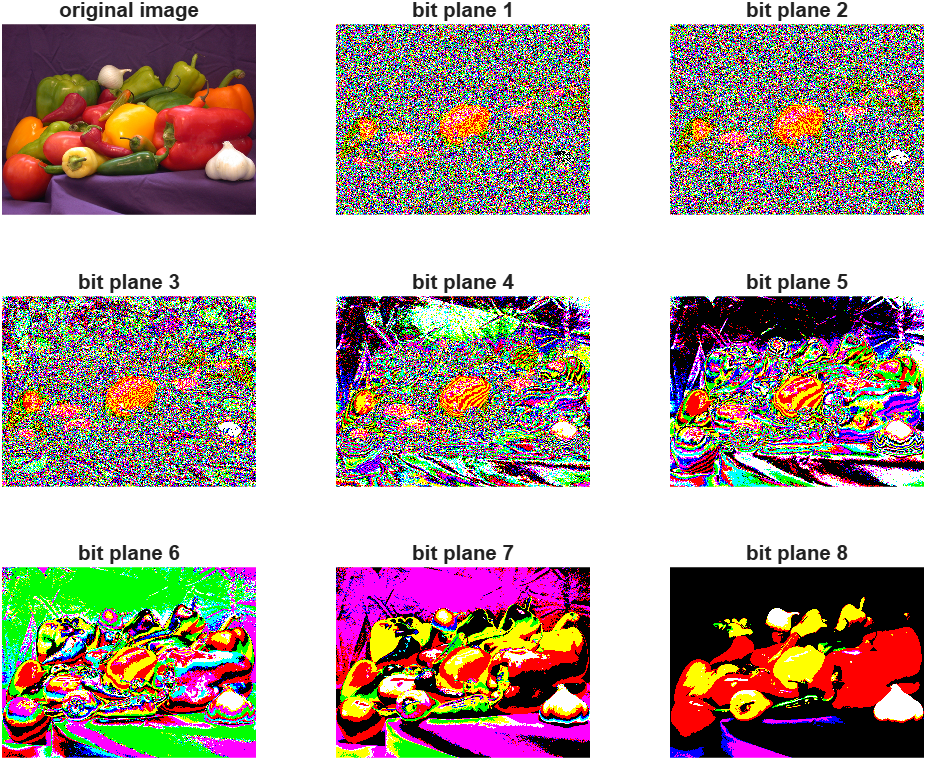
\includegraphics[width=0.65\textwidth]{Figure_2.png}
  \caption{Bit plane slicing of peppers.png: original image and bit planes.}
  \label{fig:bitplane}
\end{figure}

Figure~\ref{fig:fft} shows that the ideal LPF smooths the image by retaining
only low-frequency components (radius $D_0 = 30$), while the ideal HPF
preserves only edges by removing those same low frequencies.
Figure~\ref{fig:bitplane} shows that lower bit planes (1--3) contain mostly
noise, while higher planes (6--8) carry the dominant structural and colour
information of the image.

\end{document}
